\documentclass[tikz,border=5mm,12pt]{standalone}
\usetikzlibrary{arrows.meta}
\usetikzlibrary{decorations.pathreplacing,calligraphy}

\newcommand\edge{9mm}
\newcommand\drawpentagon{
  \draw (0,0) coordinate (P1)
    -- ++(360-36:\edge) coordinate (P2)
    -- ++(360-108:\edge) coordinate (P3)
    -- ++(180:\edge) coordinate (P4)
    -- ++(180-72:\edge) coordinate (P5)
    -- cycle;
}
\newcommand\scopexsep{24mm}
\newcommand\scopeysep{18mm}

\begin{document}
  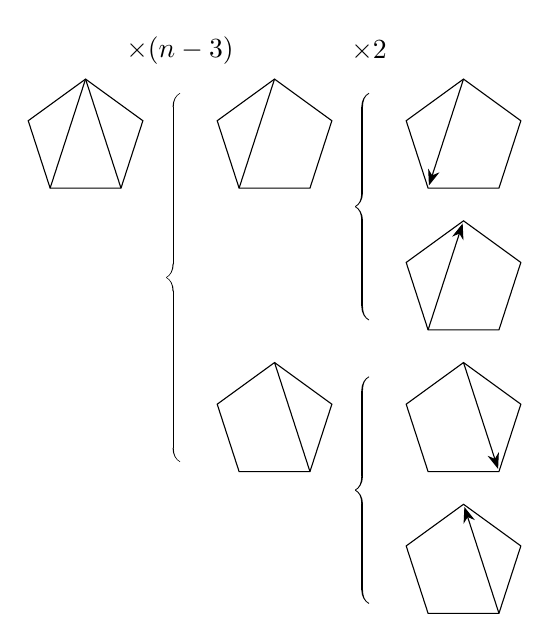
\begin{tikzpicture}[
    arr/.style={-{Stealth[length=2mm]},shorten >=1pt},
    cbrace/.style={
      decorate,
      decoration={calligraphic brace,mirror,amplitude=5pt}}
  ]
    \begin{scope}
      \drawpentagon

      \draw (P1) -- (P3);
      \draw (P1) -- (P4);
    \end{scope}

    \node at (0.5*\scopexsep,0.2*\scopeysep) {$\times (n-3)$};

    \draw[cbrace] (0.5*\scopexsep,-0.1*\scopeysep) -- ++(0,-2.6*\scopeysep);

    \begin{scope}[xshift=\scopexsep]
      \drawpentagon

      \draw (P1) -- (P4);
    \end{scope}

    \draw [cbrace,line width=0.6pt] (1.5*\scopexsep,-0.1*\scopeysep) -- ++(0,-1.6*\scopeysep);

    \begin{scope}[xshift=2*\scopexsep]
      \drawpentagon

      \draw[arr] (P1) -- (P4);
    \end{scope}

    \begin{scope}[xshift=2*\scopexsep,yshift=-\scopeysep]
      \drawpentagon

      \draw[arr] (P4) -- (P1);
    \end{scope}

    \begin{scope}[xshift=\scopexsep,yshift=-2*\scopeysep]
      \drawpentagon

      \draw (P1) -- (P3);
    \end{scope}

    \node at (1.5*\scopexsep,0.2*\scopeysep) {$\times 2$};

    \draw [cbrace,line width=0.6pt] (1.5*\scopexsep,-2.1*\scopeysep) -- ++(0,-1.6*\scopeysep);

    \begin{scope}[xshift=2*\scopexsep,yshift=-2*\scopeysep]
      \drawpentagon

      \draw[arr] (P1) -- (P3);
    \end{scope}

    \begin{scope}[xshift=2*\scopexsep,yshift=-3*\scopeysep]
      \drawpentagon

      \draw[arr] (P3) -- (P1);
    \end{scope}
  \end{tikzpicture}
\end{document}
